\section{Data and audit}
\label{sec:data}

\subsection{Dataset and split}
The data come from the October 2026 Playground episode \citep{kaggle_s6e10}.
The training set has 699{,}635 rows, the test set 299{,}844; the identifier is contiguous
across the two files (0--999{,}478) and the positive rate is 44.357\%. Twenty-one features
describe a passenger (age, flight distance, two delay columns) and a 13-item service
questionnaire answered on a 0--5 scale, plus four categorical attributes
(gender, customer type, travel type, cabin class). Three facts about the split matter for the
rest of the paper. First, an adversarial classifier that tries to separate train from test
reaches \auc{} $=0.4991$, so the two files are exchangeable and cross-validation should track
the leaderboard. Second, rating~0 is not the bottom of the scale but a code for
\emph{not applicable} (Section~\ref{sec:zero}). Third, the data are synthetic
(Section~\ref{sec:regen}).

\subsection{Label noise from discrete signatures}
\label{sec:noise}
The thirteen ratings and four categorical attributes form a coarse fingerprint: only
437{,}904 distinct signatures exist for 699{,}635 rows. Grouping by that signature separates
two kinds of rows. About half of the training rows (48.96\%) share their signature with at
least one other row; within those groups 19.76\% of rows disagree with a group member, and
flipping the minority members to the majority label would change 5.66\% of all labels.
Figure~\ref{fig:audit}a breaks this down for coarser groupings: using only the thirteen ratings
raises the conflict rate to 30.4\%, whereas adding age lowers it to 4.1\%, so the continuous
columns still carry real resolving information.

The same noise dominates the residual error of a fitted model. For the adopted model, 84.3\% of
out-of-fold predictions lie below 0.1 or above 0.9, and 4.19\% of those confident predictions
are wrong; those confident mistakes are 48.3\% of all errors. A ranker cannot repair them.

\begin{figure}[t]
\centering
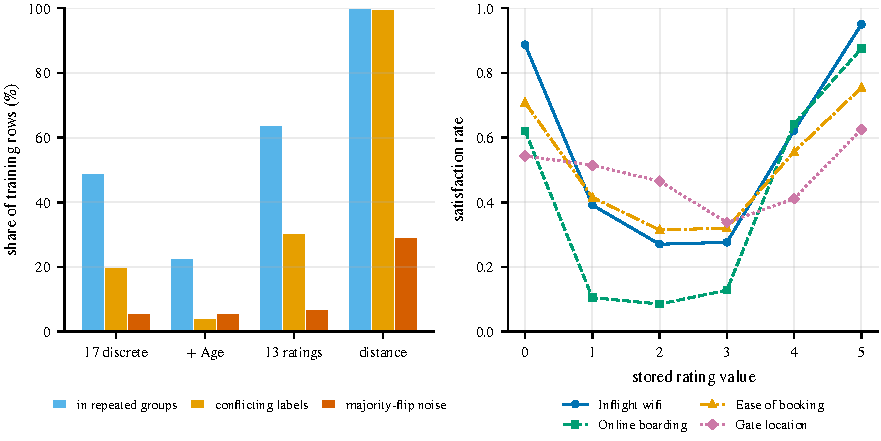
\includegraphics[width=\linewidth]{figures/fig_audit.pdf}
\caption{Left: share of training rows whose discrete signature repeats, whose labels conflict
inside such groups, and the fraction of labels that a majority vote would flip, for four
grouping keys. Right: satisfaction rate as a function of the stored rating. A stored~0 is a
``not applicable'' code, not a low score: Wi-Fi rating~0 is the \emph{most} satisfied group
(88.7\%), and every curve is non-monotone.}
\label{fig:audit}
\end{figure}

\subsection{The generator preserved distances and destroyed delays}
\label{sec:regen}
The competition data derive from a public survey of 129{,}880 passengers. Matching the two
files on the feature schema gives a precise picture of what the generator kept and what it
lost. The support of \texttt{Flight Distance} was copied almost verbatim: only 3 of the
3{,}474 distances in the training set do not occur in the survey, covering 0.0006\% of rows.
More importantly, the per-distance satisfaction rate survived: across the 2{,}243 distances
with at least 30 synthetic rows, the correlation between the synthetic and the original rate is
0.899 (Spearman 0.896), and the original rate alone scores \auc{} $=0.731$ on the synthetic
data. This is why a target encoding of the exact distance is the single most valuable feature
(Section~\ref{sec:single}): with the default \texttt{max\_bin}=255 the tree model can only
approximate 3{,}474 per-distance rates with 255 bins.

The delay columns were destroyed. In the survey, departure delay has mean 14.71 minutes and
99th percentile 180; in the synthetic data the mean is 1.18 and the 99th percentile 30, with
a point-biserial correlation of $-0.036$ against the label ($-0.051$ in the survey). Any
delay-based feature therefore has nothing to work with, which matches the negative ablation
in Figure~\ref{fig:ablation}.

\subsection{Rating zero is a missing-value code}
\label{sec:zero}
Figure~\ref{fig:audit}b shows the conditional satisfaction rate for each value of four ratings.
The curve is not monotone, and it is not noise: a Wi-Fi rating of 0 is reported by 1.87\% of
passengers and 88.7\% of them are satisfied, while a rating of 1 corresponds to 39.1\%.
Online boarding has the same shape (62.0\% at 0, 10.5\% at 1, 87.5\% at 5). Two consequences
follow. Trees can exploit the pattern with a single split at $\leq 0$, so no ``is-zero''
feature is needed (we tested it: $-0.04$ \dlt{}). A linear model, however, must see the ratings
one-hot encoded: on the same folds, logistic regression scores 0.9216 with the ratings treated
as numbers and 0.9486 with one-hot ratings, a difference of $2.7\times10^{-2}$.

\subsection{No exploitable row-level leak}
\label{sec:leak}
Because the data are synthetic, one may hope to recover the generating rows of the original
survey and inherit their labels. 27.07\% of training rows share their full 17-column signature
with a survey row, and for those rows the survey label agrees with the synthetic label 93.6\%
of the time --- but the model is better than the source: on the matched rows its \auc{} is
0.9428 while the survey label scores 0.9028, and a 50/50 blend of the two drops the overall
out-of-fold score from 0.9605 to 0.9592. We also tested for order leaks: consecutive identifiers
never share a signature, the autocorrelation of the label is smaller than $10^{-3}$, and the
mean absolute difference of flight distance between adjacent rows is 1{,}017 against 1{,}019 for
random pairs. The row order carries no information.
